
\documentclass[a4paper,11pt]{article}
\usepackage[a4paper, margin=8em]{geometry}

% usa i pacchetti per la scrittura in italiano
\usepackage[french,italian]{babel}
\usepackage[T1]{fontenc}
\usepackage[utf8]{inputenc}
\frenchspacing 

% usa i pacchetti per la formattazione matematica
\usepackage{amsmath, amssymb, amsthm, amsfonts}

% usa altri pacchetti
\usepackage{gensymb}
\usepackage{hyperref}
\usepackage{standalone}

% imposta il titolo
\title{Appunti Elettronica Digitale}
\author{Luca Seggiani}
\date{2026}

% imposta lo stile
% usa helvetica
\usepackage[scaled]{helvet}
% usa palatino
\usepackage{palatino}
% usa un font monospazio guardabile
\usepackage{lmodern}

\renewcommand{\rmdefault}{ppl}
\renewcommand{\sfdefault}{phv}
\renewcommand{\ttdefault}{lmtt}

% disponi il titolo
\makeatletter
\renewcommand{\maketitle} {
	\begin{center} 
		\begin{minipage}[t]{.8\textwidth}
			\textsf{\huge\bfseries \@title} 
		\end{minipage}%
		\begin{minipage}[t]{.2\textwidth}
			\raggedleft \vspace{-1.65em}
			\textsf{\small \@author} \vfill
			\textsf{\small \@date}
		\end{minipage}
		\par
	\end{center}

	\thispagestyle{empty}
	\pagestyle{fancy}
}
\makeatother

% disponi teoremi
\usepackage{tcolorbox}
\newtcolorbox[auto counter, number within=section]{theorem}[2][]{%
	colback=blue!10, 
	colframe=blue!40!black, 
	sharp corners=northwest,
	fonttitle=\sffamily\bfseries, 
	title=~\thetcbcounter: #2, 
	#1
}

% disponi definizioni
\newtcolorbox[auto counter, number within=section]{definition}[2][]{%
	colback=red!10,
	colframe=red!40!black,
	sharp corners=northwest,
	fonttitle=\sffamily\bfseries,
	title=~\thetcbcounter: #2,
	#1
}

% U.D.M
\newcommand{\amp}{\ensuremath{\mathrm{A}}}
\newcommand{\volt}{\ensuremath{\mathrm{V}}}
\newcommand{\meter}{\ensuremath{\mathrm{m}}}
\newcommand{\second}{\ensuremath{\mathrm{s}}}
\newcommand{\farad}{\ensuremath{\mathrm{F}}}
\newcommand{\henry}{\ensuremath{\mathrm{H}}}
\newcommand{\siemens}{\ensuremath{\mathrm{S}}}

% circuiti
\usepackage{circuitikz}
\usetikzlibrary{babel}

% disegni
\usepackage{pgfplots}
\pgfplotsset{width=10cm,compat=1.9}

% disponi codice
\usepackage{listings}
\usepackage[table]{xcolor}

\definecolor{codegreen}{rgb}{0,0.6,0}
\definecolor{codegray}{rgb}{0.5,0.5,0.5}
\definecolor{codepurple}{rgb}{0.58,0,0.82}
\definecolor{backcolour}{rgb}{0.95,0.95,0.92}

\lstdefinestyle{codestyle}{
		backgroundcolor=\color{black!5}, 
		commentstyle=\color{codegreen},
		keywordstyle=\bfseries\color{magenta},
		numberstyle=\sffamily\tiny\color{black!60},
		stringstyle=\color{green!50!black},
		basicstyle=\ttfamily\footnotesize,
		breakatwhitespace=false,         
		breaklines=true,                 
		captionpos=b,                    
		keepspaces=true,                 
		numbers=left,                    
		numbersep=5pt,                  
		showspaces=false,                
		showstringspaces=false,
		showtabs=false,                  
		tabsize=2
}

\lstdefinestyle{shellstyle}{
		backgroundcolor=\color{black!5}, 
		basicstyle=\ttfamily\footnotesize\color{black}, 
		commentstyle=\color{black}, 
		keywordstyle=\color{black},
		numberstyle=\color{black!5},
		stringstyle=\color{black}, 
		showspaces=false,
		showstringspaces=false, 
		showtabs=false, 
		tabsize=2, 
		numbers=none, 
		breaklines=true
}

\lstdefinelanguage{javascript}{
	keywords={typeof, new, true, false, catch, function, return, null, catch, switch, var, if, in, while, do, else, case, break},
	keywordstyle=\color{blue}\bfseries,
	ndkeywords={class, export, boolean, throw, implements, import, this},
	ndkeywordstyle=\color{darkgray}\bfseries,
	identifierstyle=\color{black},
	sensitive=false,
	comment=[l]{//},
	morecomment=[s]{/*}{*/},
	commentstyle=\color{purple}\ttfamily,
	stringstyle=\color{red}\ttfamily,
	morestring=[b]',
	morestring=[b]"
}

% disponi sezioni
\usepackage{titlesec}

\titleformat{\section}
	{\sffamily\Large\bfseries} 
	{\thesection}{1em}{} 
\titleformat{\subsection}
	{\sffamily\large\bfseries}   
	{\thesubsection}{1em}{} 
\titleformat{\subsubsection}
	{\sffamily\normalsize\bfseries} 
	{\thesubsubsection}{1em}{}

% disponi alberi
\usepackage{forest}

\forestset{
	rectstyle/.style={
		for tree={rectangle,draw,font=\large\sffamily}
	},
	roundstyle/.style={
		for tree={circle,draw,font=\large}
	}
}

% disponi algoritmi
\usepackage{algorithm}
\usepackage{algorithmic}
\makeatletter
\renewcommand{\ALG@name}{Algoritmo}
\makeatother

% disponi numeri di pagina
\usepackage{fancyhdr}
\fancyhf{} 
\fancyfoot[L]{\sffamily{\thepage}}

\makeatletter
\fancyhead[L]{\raisebox{1ex}[0pt][0pt]{\sffamily{\@title \ \@date}}} 
\fancyhead[R]{\raisebox{1ex}[0pt][0pt]{\sffamily{\@author}}}
\makeatother

\begin{document}
% sezione (data)
\section{Lezione del 13-03-26}

% stili pagina
\thispagestyle{empty}
\pagestyle{fancy}

% testo
\subsection{Diodi}
Le giunzioni P/N come le abbiamo studiate nell'ultima lezione formano quei componenti elettronici noti come \textbf{diodi}, col simbolo del componente circuitale:
\begin{center}
	\begin{circuitikz}
	\node at (0,0) [anchor=south] {$+, A$};
	\node at (3,0) [anchor=south] {$-, K$};
	\draw (0,0) to[D] (3,0);
	\end{circuitikz}
\end{center}
vediamo come si prende la corrente $I_D$ come la corrente lungo il diodo, da $+$ (anodo $A$) a $-$ (catodo $K$), e il voltaggio $V_d$ come quello che si trova fra $+$ e $-$.

I diodi sono governati dalla cosiddetta legge di \textit{Shockley}:
\begin{definition}{Legge di Shockley}
La corrente $I_D$ su un diodo sottoposto a tensione $V_D$ dipende da:
$$
I_D = I_S \left( e^\frac{V_D}{\eta V_T} - 1 \right)
$$
\end{definition}
dove $I_S$ è la \textit{corrente inversa di saturazione}, $\eta$ è il \textit{fattore di idealità}, e $V_T$ è la tensione termica:
$$
V_T = \frac{k_B T}{e}
$$
già vista nella legge di Einstein a 4.3, e già usata per il calcolo del potenziale "built-in" della giunzione P/N in 5.1.

Tracciamo quindi il grafico tensione-corrente del diodo, prendendo i seguenti intervalli:
\begin{itemize}
	\item Per $V_D = 0$, avremo $I_D = 0$;
	\item Per $V_D$ positivo, il termine esponenziale domina, e si ha:
		$$
		I_D \approx I_S e^{\frac{V_D}{\eta V_T}}
		$$
	cioè la crescita è sostanzialmente esponeziale;
	\item Per $V_D$ negativo, il termine esponenziale è molto piccolo, e si ha:
		$$
		I_D \approx -I_s
		$$
		Col fatto che $I_s$ è solitamente molto piccola (intorno a $10^{-10} \, \mathrm{A}$), si ha quindi che il valore di $I_D$ per $V_D < 0$ è piccolo e costante.
\end{itemize}

\begin{center}
	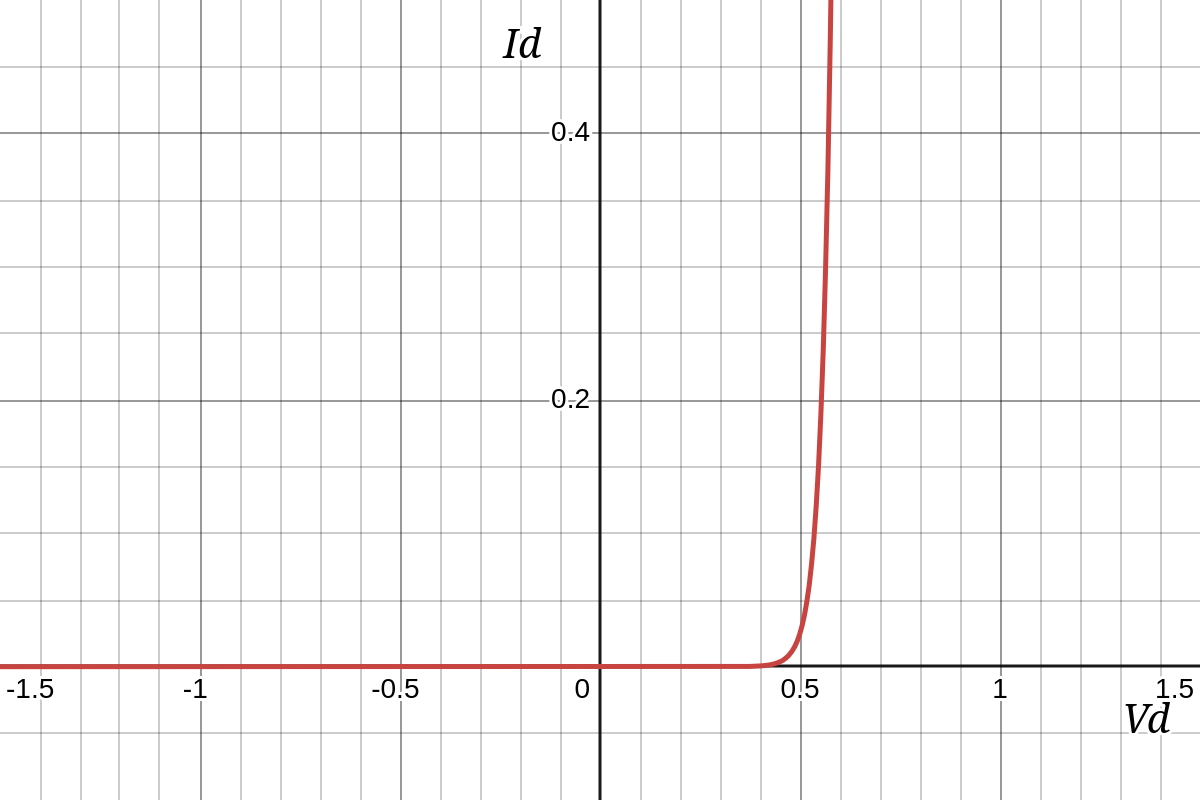
\includegraphics[scale=0.28]{../figures/diode.png}
\end{center}

Abbiamo quindi visto il comportamento tipico del diodo, che è chiaramente un componente \textit{non lineare}: per $V_D > 0$ a cui si sottopone il diodo, la corrente cresce in maniera esponenziale, mentre per $V_D < 0$ quasi non passa corrente. Possiamo dire che, in nqualche modo, il diodo "rettifica" la corrente che ci passa. 

\subsubsection{Saturazione e breakdown}
Vediamo alcuni fenomeni particolari che il diodo presenta agli estremi di tensione:
\begin{itemize}
	\item 
Notiamo subito che la legge esponenziale per $V_D > 0$ non è soddisfatta in assoluto: esiste una certa soglia massima di \textbf{saturazione}, oltre la quale $I_D$ resta costante o addirittura decresce.
	\item
Per il caso opposto, cioè $V_D < 0$, il diodo entra in una fase di cosiddetto \textbf{breakdown} (reversibile). Abbiamo infatti che a $V_D$ molto negativi, oltre una certa soglia la corrente passa da $I_S$ costante ad un valore esponenzialmente grande, cioè una grande corrente si trova a scorrere sul diodo. Per questo motivo, spesso si mettono resistenze in serie ai diodi, in modo da evitare di superare i limiti di potenza nel caso di fenomeni di breakdown.

Per spiegarci tale fenomeno, ricordiamo che la corrente in polarizzazione inversa è principalmente una corrente di drift, cioè causa dei portatori minoritari di ciascuna regione (P ed N) che viaggiano lungo il potenziale "built-in" (formato sulla giunzione dagli ioni fissi), aumentato dal potenziale di polarizzazione.
Dovrà quindi esistere un qualche fenomeno che aumenta il numero di portatori minoritari a grandi valori di $V_D$. In verità questi effetti sono due:
\begin{itemize}
	\item Effetto \textbf{Zener}: in opportune situazioni di drogaggio, il campo elettrico nella zona di svuotamento è abbastanza forte da rompere alcuni legami covalenti, portando alla formazione di nuovi portatori;
	\item Effetto \textbf{valanga}: gli elettroni in moto nella giunzione P/N possono fornire energia tale agli atomi contro cui collidono da liberare altri atomi (\textit{ionizzazione per urto}). In particolare, vediamo che se partiamo con un elettrone $e_0$, dopo un urto otteniamo 2 nuovi portatori ($e_1$ e la relativa lacuna $h1$). Entrambi di questi portatori (anche la lacuna, ma chiaramente spostandosi in direzione opposta: questo potrebbe sembrare strano, ma dobbiamo pensare alle lacune come particelle positive, dove l'energia immagazzinata è quella che viene tolta agli elettroni che vengono spostati) possono quindi continuare a collidere e a generare nuovi portatori. Questo fenomeno ha quindi crescita esponenziale, cioè all $i$-esimo urto partendo da un solo elettrone $e_0$ si hanno:
		$$
		[e, p] = 3^i
		$$
		portatori di carica.
\end{itemize}

Esistono particolari tipi di diodi, detti \textbf{diodi Zener}, che sfruttano l'effetto di breakdown. Il loro simbolo del componente circuitale è:
\begin{center}
	\begin{circuitikz}
	\node at (0,0) [anchor=south] {$+$};
	\node at (3,0) [anchor=south] {$-$};
	\draw (0,0) to[zD] (3,0);
	\end{circuitikz}
\end{center}
e la loro caratteristica è che l'effetto di breakdown avviene a tensioni molto più piccole del normale (ordine di $100 \, \mathrm{V}$ nei diodi normali, ordine dei $10 \, \mathrm{V}$ o meno nei diodi Zener). 
Spesso i diodi Zener vengono fatti lavorare nella loro zona di breakdown, in quanto in questo modo possono fare da riferimento per la tensione (se la curva di corrente in fase di breakdown fosse perfettamente verticale, sarebbero effettivamente generatori di tensione).
\end{itemize}

\subsubsection{Temperatura nei diodi}
Vediamo qual'è l'effetto della temperatura sul comportamento dei diodi.
\begin{itemize}
	\item Nel caso di diodi ad effetto \textit{Zener}, all'aumentare della temperatura $T$ la tensione di breakdown $V_{BR}$ aumenta (cioè l'effetto di breakdown avviene ad una tensione maggiore);
	\item Nel caso di diodi ad effetto \textit{Valanga}, prendiamo in considerazione il fatto che se si aumenta $T$ la mobilità elettronica $\mu_n$ e di lacuna $\mu_p$ diminuiscono (aumenta la frequenza degli urti).

		Potremmo pensare che questo porti ad un maggiore effetto valanga, ma il risultato effettivo è che il tempo di cammino medio $\tau$, e quindi la lunghezza del cammino medio stesso (abbiamo parlato di cammini liberi discutendo il modello di Drude-Lorentz in 2.1.2), diminuiscono, per cui diminuisce l'energia che i portatori riescono ad accumulare e quindi trasferire agli atomi in fase di urto.
		Il risultato è quindi che la tensione di breakdown $V_{BR}$ diminuisce (cioè l'effetto di breakdown avviene ad una tensione minore).
\end{itemize}

Esistono diodi particolari, all'interno della famiglia dei diodi Zener, costruiti per presentare entrambi gli effetti. Solitamente infatti si ha che:
\begin{itemize}
	\item I diodi che stanno fra $0$ e $5$ volts di tensione di breakdown $V_{BR}$ presentano principalmente l'effetto Zener;
	\item I diodi che stanno fra $7$ e $+\infty$ volts di tensione di breakdown $V_{BR}$ presentano principalmente l'effetto Zener;
	\item I diodi che stanno nella regione di mezzo (fra $5$ e $7$ volts) della tensione di breakdown $V_{BR}$ presentano principalmente entrambi gli effetti. Il risultato è che i 2 effetti in qualche modo si bilanciano, e la tensione $V_{BR}$ resta perlopiù costante. Questo è utile nel caso di diodi Zener che, come abbiamo detto nella scorsa sezione, servono a fare da riferimento di tensione. 
\end{itemize}

\subsubsection{Circuito RD}
Vediamo quindi il diodo da un punto di vista circuitale, risolvendo un semplice circuito, formato da un resistore in serie ad un diodo:
\begin{center}
	\begin{tikzpicture}
		\draw (0,0) to [ voltage source,  l=$V_A$] (0,3)
			to [ resistor, l=$R$] (3,3)
			to [ diode] (3,0)
			-- (0,0);
		\node at(3,2.25) [anchor=west] {$A$};
		\node at(3,0.75) [anchor=west] {$K$};
	\end{tikzpicture}
\end{center}

In casi come questo, visto che si parla di componenti non lineari, molti dei teoremi e delle leggi che conosciamo dall'elettrotecnica non valgono più. Dobbiamo quindi trovare dei metodi di soluzione alternativi.

\begin{itemize}
	\item \textbf{\textsf{Metodo numerico}} \\
Anche se non valgono più molti teoremi, valgono sempre, invece, le leggi di analisi circuitale di Kirchoff (viste nella lezione 3). Imponendo ad esempio la seconda legge sulla maglia del circuito si ha:
\[
	\begin{cases}
		V_A = R I_D + V_D \\ 
		I_D = I_s \left( e^\frac{V_D}{\eta V_T} - 1 \right)
	\end{cases}
\]

Questo sistema è però fortemente non lineare (presenta una funzione esponenziale), ed è quindi adatto particolarmente a metodi \textit{numerici} (anche se questo piccolo esempio è risolvibile, circuiti più complessi con più diodi probabilmente non lo saranno). Per questo motivo, lo chiamiamo metodo \textbf{numerico}. 

	\item \textbf{\textsf{Metodo grafico}} \\
Una possibile soluzione, in casi semplici, è data dal metodo grafico. Potremo infatti ricavare $I_D$ da entrambi le equazioni dello scorso sistema:
\[
	\begin{cases}
		I_D = \frac{V_A - V_D}{R} \\ 
		I_D = I_s \left( e^\frac{V_D}{\eta V_T} - 1 \right)
	\end{cases}
\]
cioè rispettivamente ottenere una retta ed un esponenziale, che potremo quindi interesecare su un grafico per trovare valori approssimati di $I_D$ al particolare $V_D$ (formando la coppia ($(V_{DQ}, I_{DQ})$) che risolve il sistema).
\begin{center}
	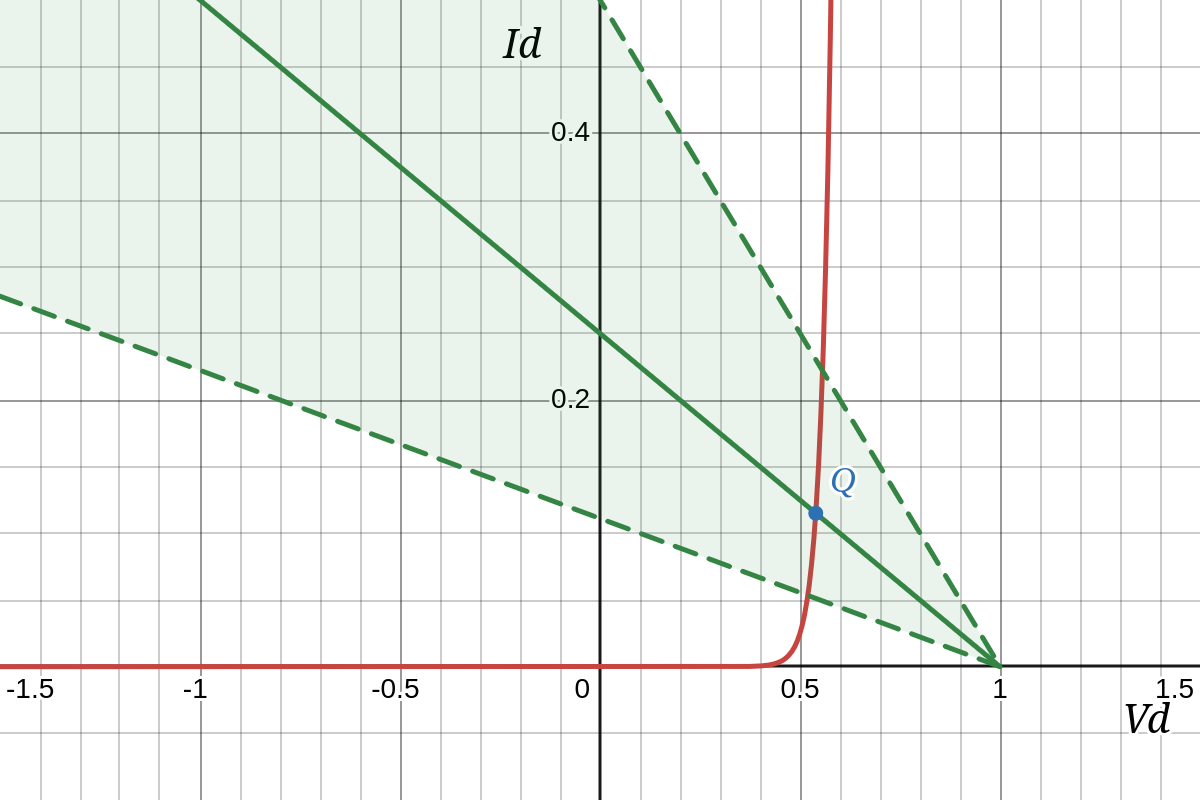
\includegraphics[scale=0.28]{../figures/rd_graph.png}
\end{center}
Questo punto di intersezione viene detto punto di \textbf{lavoro} o di \textit{quiescenza}, ed indicato con $Q$.

Notiamo che la retta:
$$
I_D = \frac{V_A - V_D}{R} \\ 
$$
dove $V_A$ è il potenziale esterno e $V_D$ è quello sul diodo, viene chiamata \textbf{retta di carico} (e l'intero metodo prende anche il nome di \textit{metodo della retta di carico}).

Sempre dal grafico, notiamo che variando $R$ si ottengono diversi grafici della retta di carico, che mostrano direttamente la variazione della corrente al punto di quiescenza $Q$. In particoare:
\begin{itemize}
	\item Al diminuire di $R$, si ottiene una retta del fascio con coefficiente angolare più grande (in modulo), e quindi si interseca un punto più alto della curva di Shockley (maggiore corrente $I_D$ sul diodo);
	\item All'aumentare di $R$, si ottiene una retta del fascio con coefficiente angolare più piccolo (in modulo), e quindi si interseca un punto più basso della curva di Shockley (mnore corrente $I_D$ sul diodo);
\end{itemize}

\item \textbf{\textsf{Metodo approssimato}} \\
Notiamo che gli ultimi due metodi che abbiamo visto (metodo \textit{numerico} e metodo \textit{grafico}) sono metodi \textit{non approssimati} e quindi esatti (che per noi significa ad altissima precisione). Vediamo quindi che esistono metodi ad alta precisione, ma approssimati, che rinunciano alla legge di Shockley (che non sappiamo risolvere) e quindi danno vita a sistemi risolvibili.
Questi vengono detti modelli del diodo per \textbf{grandi segnali}.

\end{itemize}

\subsubsection{Modelli del diodo per grandi segnali}
Vediamo quindi quali sono questi 3 modelli approssimati del diodo per \textit{grandi segnali}.

\begin{itemize}
\item \textbf{\textsf{Modello a caduta costante}} \\
Nel modello a \textbf{caduta costante} sfruttiamo il fatto che $I_D$ è quasi nulla per $V_D$ minore di una certa soglia (solitamente $V_\gamma = 0.7 \, \mathrm{V}$). 
Prendiamo quindi il diodo come un circuito \textit{aperto} al di sotto di tale soglia ($V_D < V_\gamma$), e di li in poi ($V_D > V_\gamma$) lo approssimiamo come un \textit{generatore di tensione} (qualsiasi corrente alla stessa tensione, cioè sul grafico una linea verticale). 
\begin{center}
	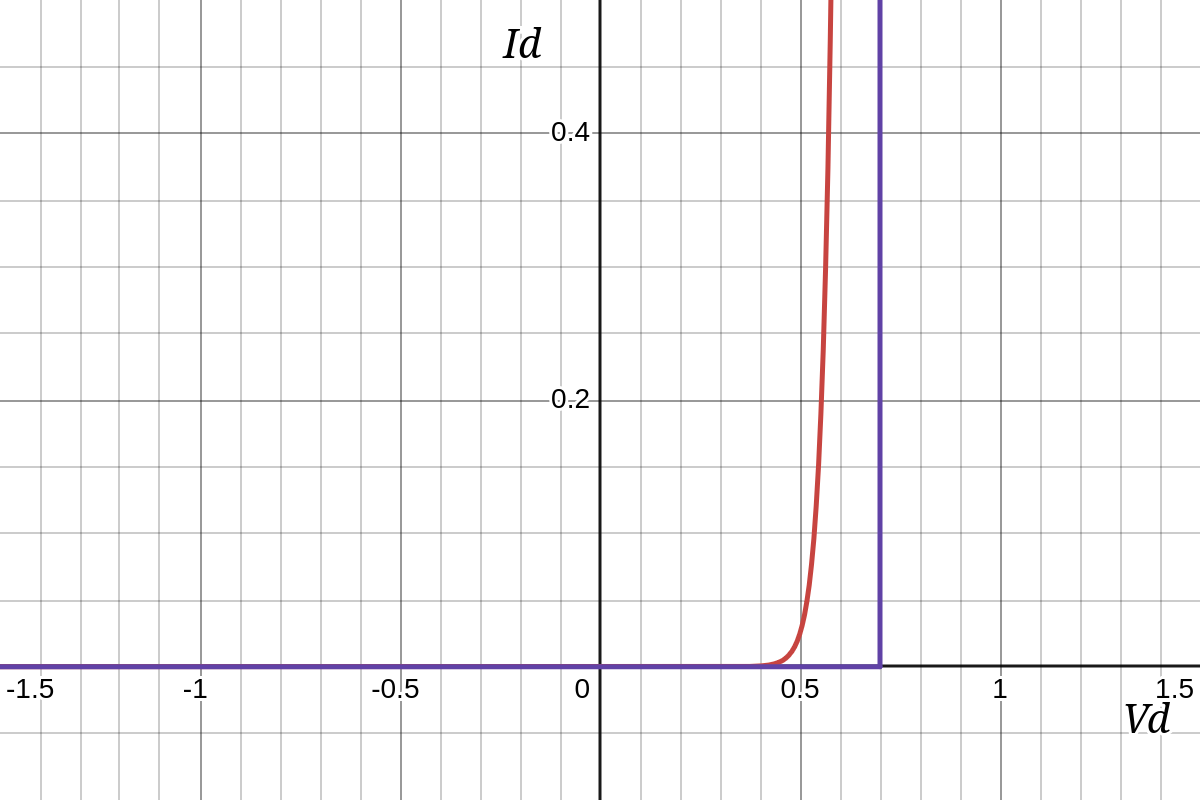
\includegraphics[scale=0.25]{../figures/caduta_diode.png}
\end{center}

Dal punto di vista dei calcoli, un modello di questo tipo (sostanzialmente binario) si risolve facendo una prima ipotesi riguardo al regime di comportamento del diodo (aperto o generatore di tensione), quindi risolvendo il circuito, e controllando se il risultato è fisicamente valido. Se non lo è, chiaramente l'ipotesi da fare sarà stata l'altra.

Questo si può fare grazie al \textit{teorema dei circuiti}:
\begin{theorem}{Teorema dei circuiti}
	Che in un circuito ci siano elementi lineari e non, se questi hanno tutti andamento monotono crescente, esiste una e una sola soluzione del circuito.
\end{theorem}

Notiamo però che questo metodo diventa difficile da applicare per molti diodi, in quanto si hanno 2 opzioni per diodo, che risultano in $2^n$ possibilità di ipotesi iniziali per $n$ diodi.

\item \textbf{\textsf{Modello del diodo ideale}} \\
Questo modello equivale a quello della caduta costante, ma con $V_\gamma$ preso nullo. Questo significa che per $V_D < 0$ il diodo modellizzato si comporterà come un circuito \textit{aperto}, mentre per $V_D > 0$ si comporterà come un circuito aperto. Notiamo che per fare questo, trascuriamo completamente la caduta di potenziale sul diodo: in questo il modello del diodo ideale è più semplice di quello a caduta costante (risulta valido in circuiti dove le cadute di potenziale sono più grandi di quelle del diodo, cioè di $V \approx 0.7 \, \mathrm{V}$).
\begin{center}
	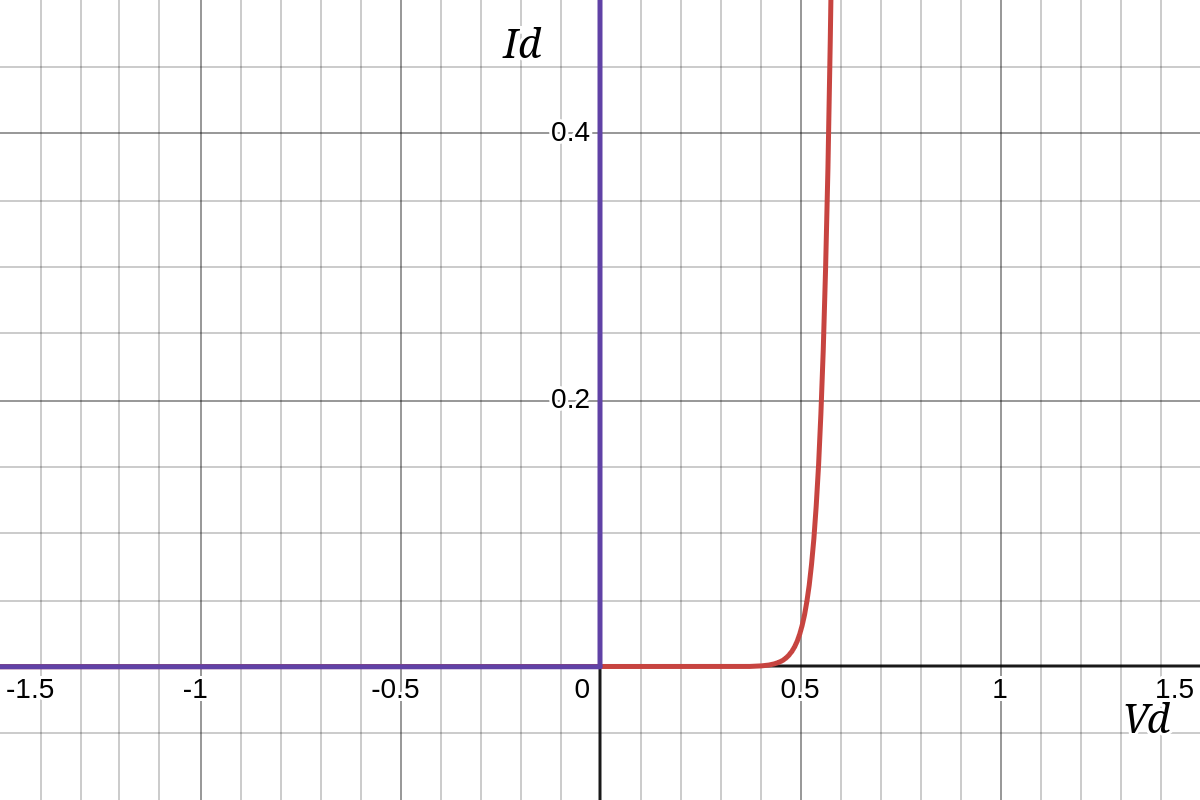
\includegraphics[scale=0.25]{../figures/ideale_diode.png}
\end{center}

Dal punto di vista dei calcoli, un modello di questo tipo è sempre binario, e si risolve facendo una prima ipotesi riguardo al regime di comportamento del diodo (aperto o cortocircuito), quindi risolvendo il circuito, e controllando se il risultato è fisicamente valido. Se non lo è, chiaramente l'ipotesi da fare sarà stata l'altra.

\item \textbf{\textsf{Modello lineare a tratti}} \\
	In questo caso cerchiamo un approssimazione migliore della caduta costante, lineare, che cerchi di "inseguire" in qualche modo l'andamento dell'esponenziale, almeno vicino a $V_\gamma \approx 0.7 \, \mathrm{V}$. In questo caso, per $V_D < V_\gamma$, il diodo modellizzato si comporta sempre come un circuito \textit{aperto}, mentre per $V_D > V_\gamma$ si comporta come una serie \textit{generatore di tensione - resistenza}. 

\begin{center}
	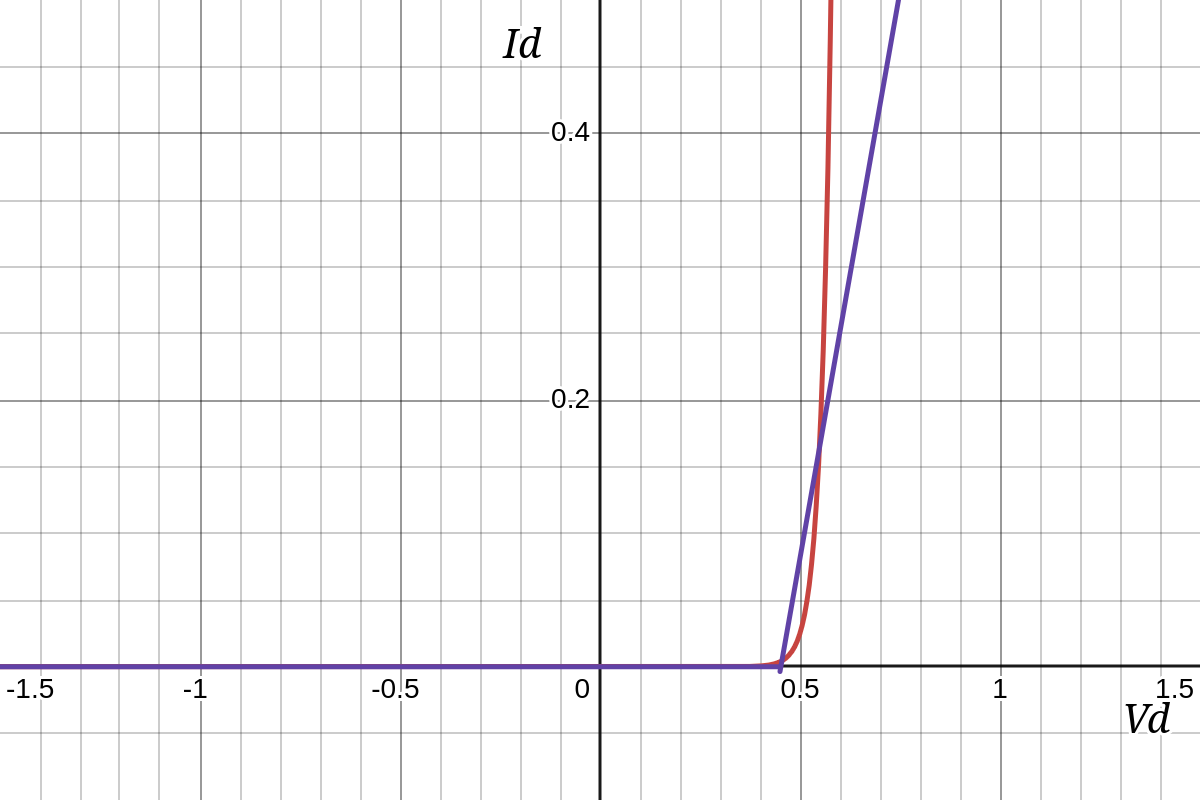
\includegraphics[scale=0.25]{../figures/lineare_diode.png}
\end{center}

Dal punto di vista dei calcoli questo modello è analogo ai precedenti, ma presenta delle complessità maggiori: andiamo a sostituire il diodo (che è un solo componente circuitale) con 2 componenti (generatore di tensione e resistenza), cosa che comporta una grande complicazione di circuiti con molti diodi. 

\end{itemize}

\end{document}
